
\documentclass{beamer}

\usepackage{algpseudocode, color, colortbl, listings, MnSymbol}

\usepackage{hyperref}
\hypersetup{
    colorlinks=true,
    urlcolor=blue,
}

\usepackage{tikz, xcolor}

\usetheme{Montpellier}
\usecolortheme{rose}

% page numbers, from
% https://tex.stackexchange.com/questions/137022/how-to-insert-page-number-in-beamer-navigation-symbols
\expandafter\def\expandafter\insertshorttitle\expandafter{%
  \insertshorttitle\hfill%
  \insertframenumber\,/\,\inserttotalframenumber}

\definecolor{Gray}{gray}{0.8}
\newcolumntype{g}{>{\columncolor{Gray}}c}

\newcommand{\stanza}{ \\~\ }

\title{15. Convex Hulls}
\subtitle{CPSC 535}
\author{Kevin A. Wortman}
\institute{ 
\includegraphics[height=2cm]{csuf-logo-cmyk} }
\date{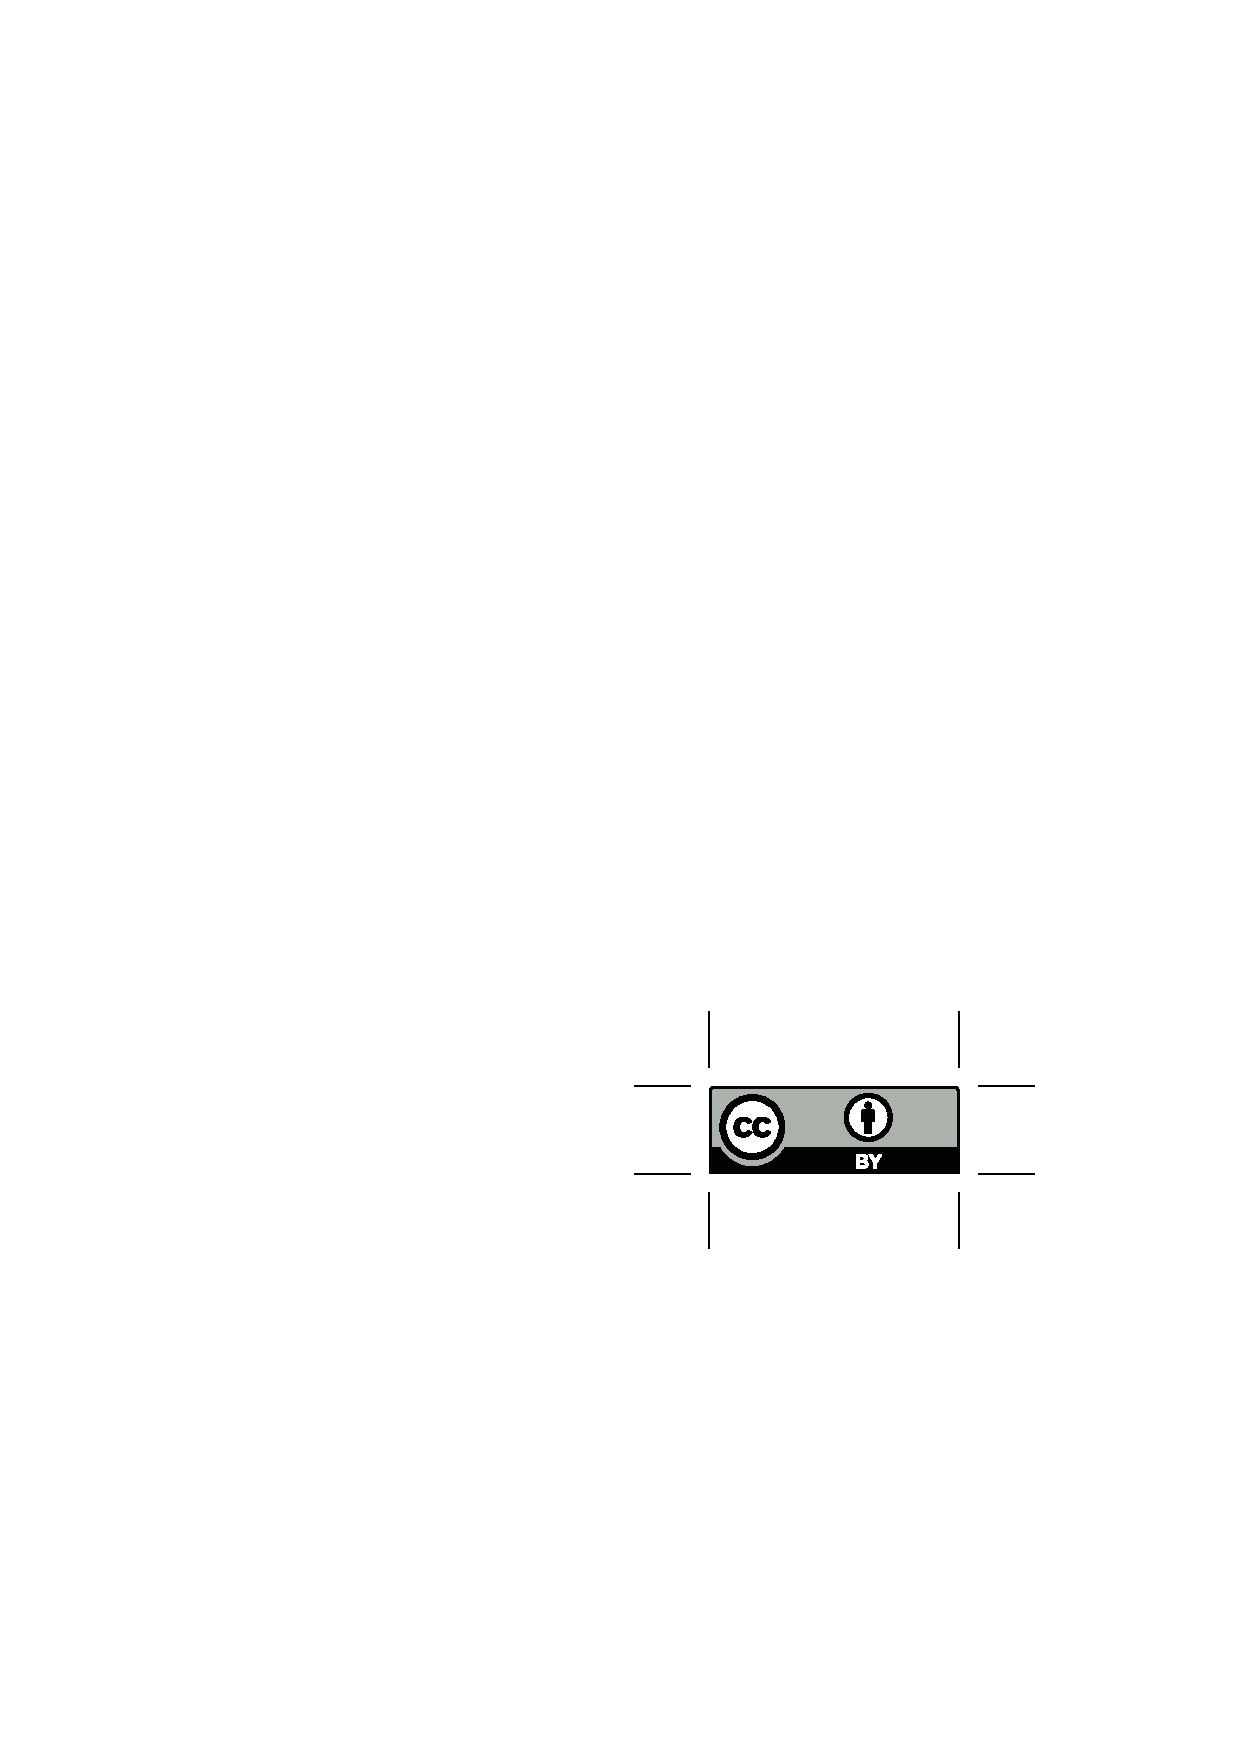
\includegraphics[height=14pt]{by} \\

{\tiny
This work is licensed under a
\href{http://creativecommons.org/licenses/by/4.0/}{Creative Commons Attribution 4.0 International License}.
}}

\begin{document}

\begin{frame}
  \titlepage
\end{frame}

\begin{frame} \frametitle{Convex Hulls}
\emph{convex hull problem} \\
\textbf{input}: set of $n \geq 3$ points $Q$ \\
\textbf{output}: $CH(Q)$, the subset of $Q$ that is the set of vertices on
  the convex hull of $Q$ \stanza

convex hull $\equiv$ boundary of convex polygon enclosing all of $Q$\\
  \begin{center}
    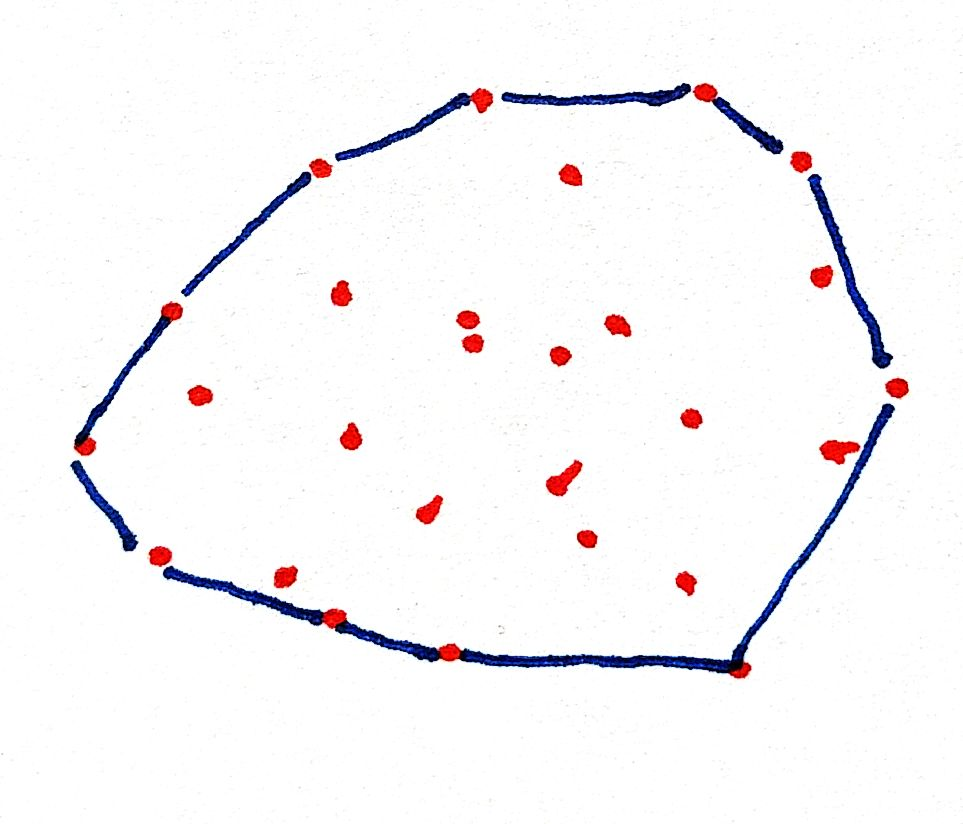
\includegraphics[width=4cm]{convex_hull.jpg}
  \end{center}
\end{frame}

\begin{frame} \frametitle{Convex Hull Applications}
\begin{itemize}
  \item object intersection in raytracing, video games, GUIs
  \item drawing implicit regions in GIS
  \item finding farthest points (they're always $CH$ vertices)
  \item component of other algorithms
\end{itemize}
\end{frame}

\begin{frame} \frametitle{Approaches to Convex Hulls}
Like the sorting problem, many algorithm patterns work for convex hulls,
and there is a rich literature of competitive algorithms. \stanza

\begin{itemize}
  \item Greedy pattern: line-sweep, update hull as we go
  \item Divide-and-conquer: divide $Q$ in half, compute convex hulls for each
    half, merge two convex hulls into one
  \item Iterative improvement: start with a superset of $CH(Q)$; refine by repeatedly eliminating
    a constant fraction of the points until only $CH(Q)$ remains
\end{itemize}
\end{frame}

\begin{frame} \frametitle{Baseline Algorithm}
\textbf{Observe}
\begin{itemize}
  \item any two input points define a line $\ell$
  \item when those points are both in $CH(Q),$ remaining $n-2$ points are all on
    the same side of $\ell$ \textbf{(a geometric property)}
  \item $\implies$ for each pair of input points $p, q$, see whether all other points
    are on the same side of $\ell$
  \item if so include $p, q$ in $CH(Q)$
\end{itemize}
\end{frame}

\begin{frame} \frametitle{Baseline Algorithm}
  \begin{center}
    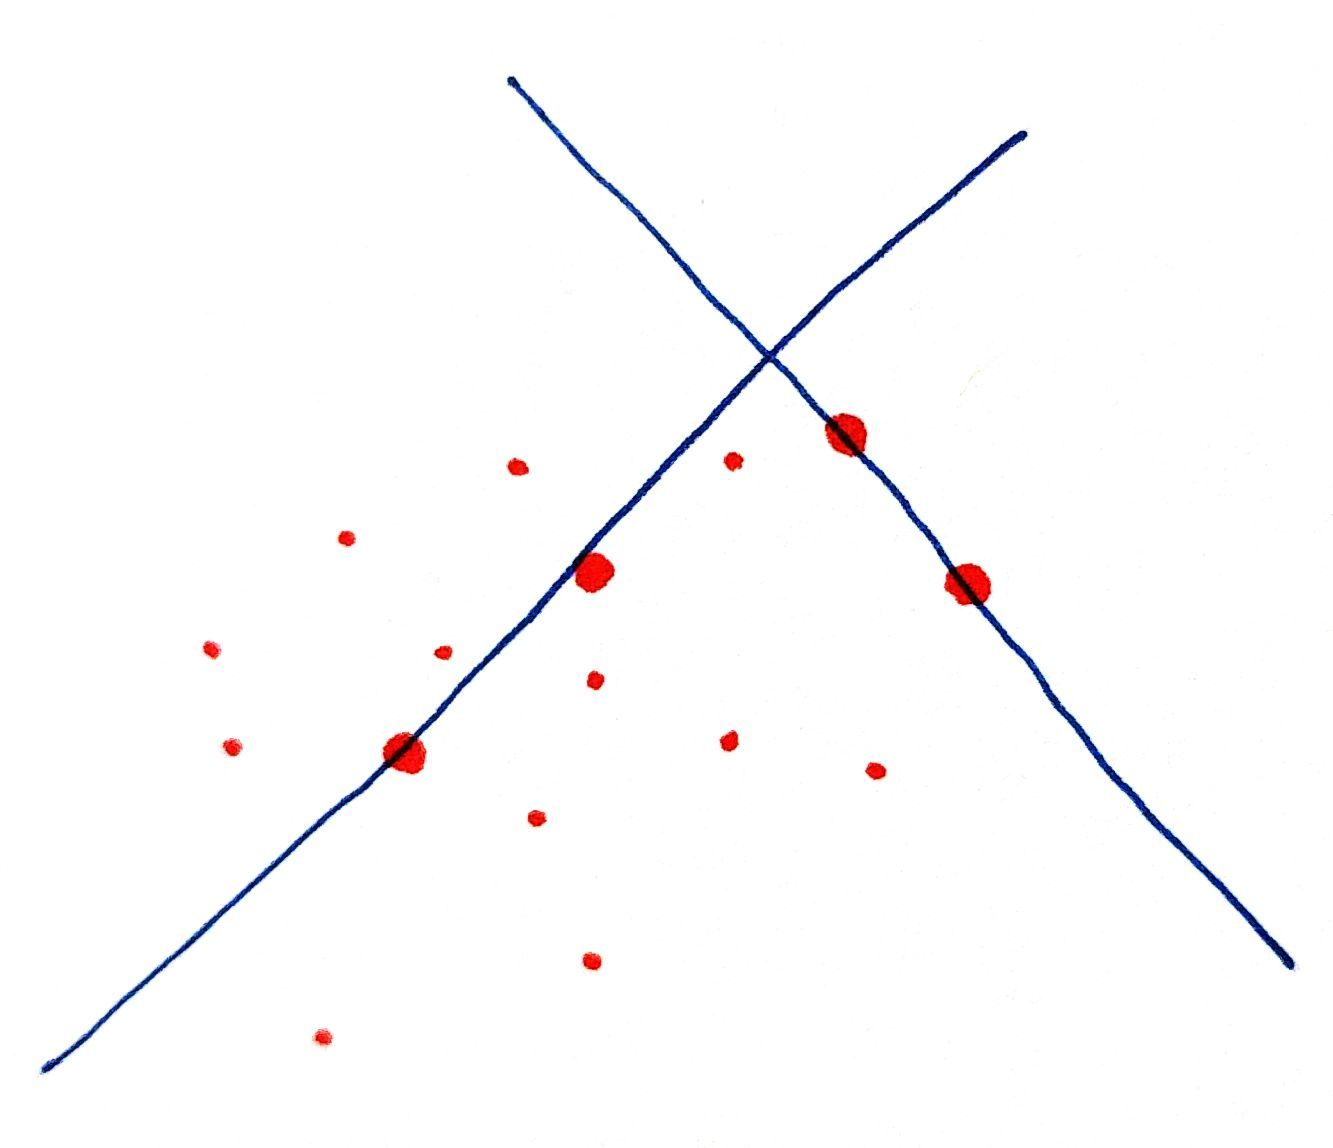
\includegraphics[width=6cm]{convex_hull_line.jpg}
  \end{center}
\end{frame}
  
\begin{frame} \frametitle{Baseline Pseudocode}
  {\small
\begin{algorithmic}[1]
  \Function{NAIVE-CONVEX-HULL}{$Q$}
    \State $H=\emptyset$
    \For { distinct points $p, q \in Q$ }
      \State form line $\ell$ intersecting $p$ and $q$
      \State $k = $ \# points above $\ell$
      \If { $k=(n-2)$ or $k=0$ }
        \State $H = H \cup \{p, q\}$
      \EndIf
    \EndFor
    \State \Return $H$
  \EndFunction \stanza
\end{algorithmic}
}

\textbf{Analysis}: $\Theta(n^2)$ iterations, counting \#points is $\Theta(n)$ \\
$\Longrightarrow \Theta(n^3)$ time
\end{frame}

\begin{frame} \frametitle{Graham Scan Idea}
\begin{itemize}
  \item greedy pattern, reduction-to-sorting
  \item \textbf{Geometric property}: when touring a CH in counter-clockwise order, we
    \textbf{only make left turns}
  \item right turn $=$ exiting a concavity, middle point not in hull
  \item $\therefore$ sweep counter-clockwise, keep points that participate in left
    turns, drop points in the middle of right turns 
  \item alternative kind of line sweep: rotating the line (not left-to-right)
\end{itemize}
\end{frame}

\begin{frame} \frametitle{Graham Scan Idea}
  \begin{center}
    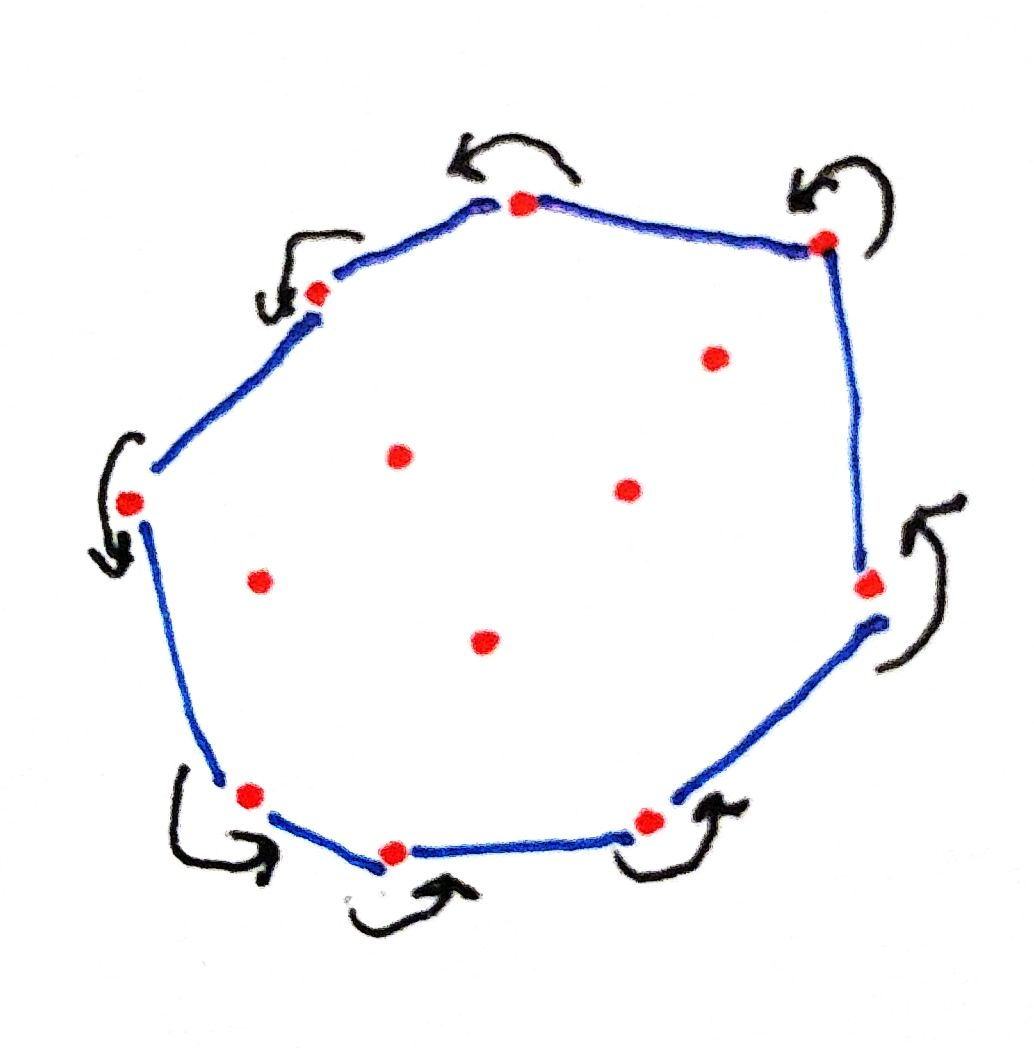
\includegraphics[width=4cm]{convex_hull_left_turns.jpg}
    \hspace{.5cm}
    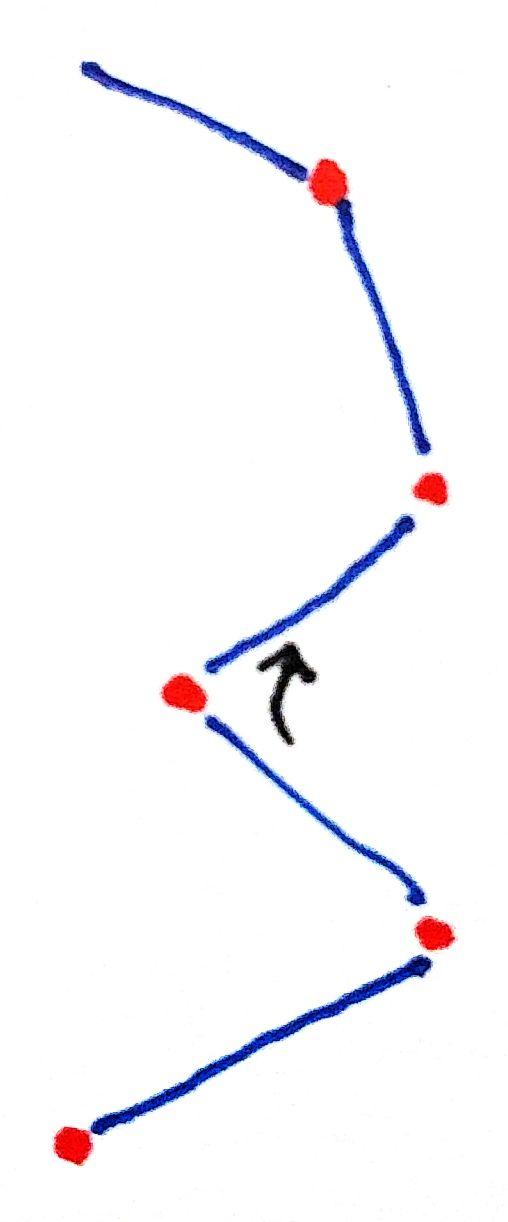
\includegraphics[height=4cm]{convex_hull_concavity.jpg}
    \hspace{.5cm}
    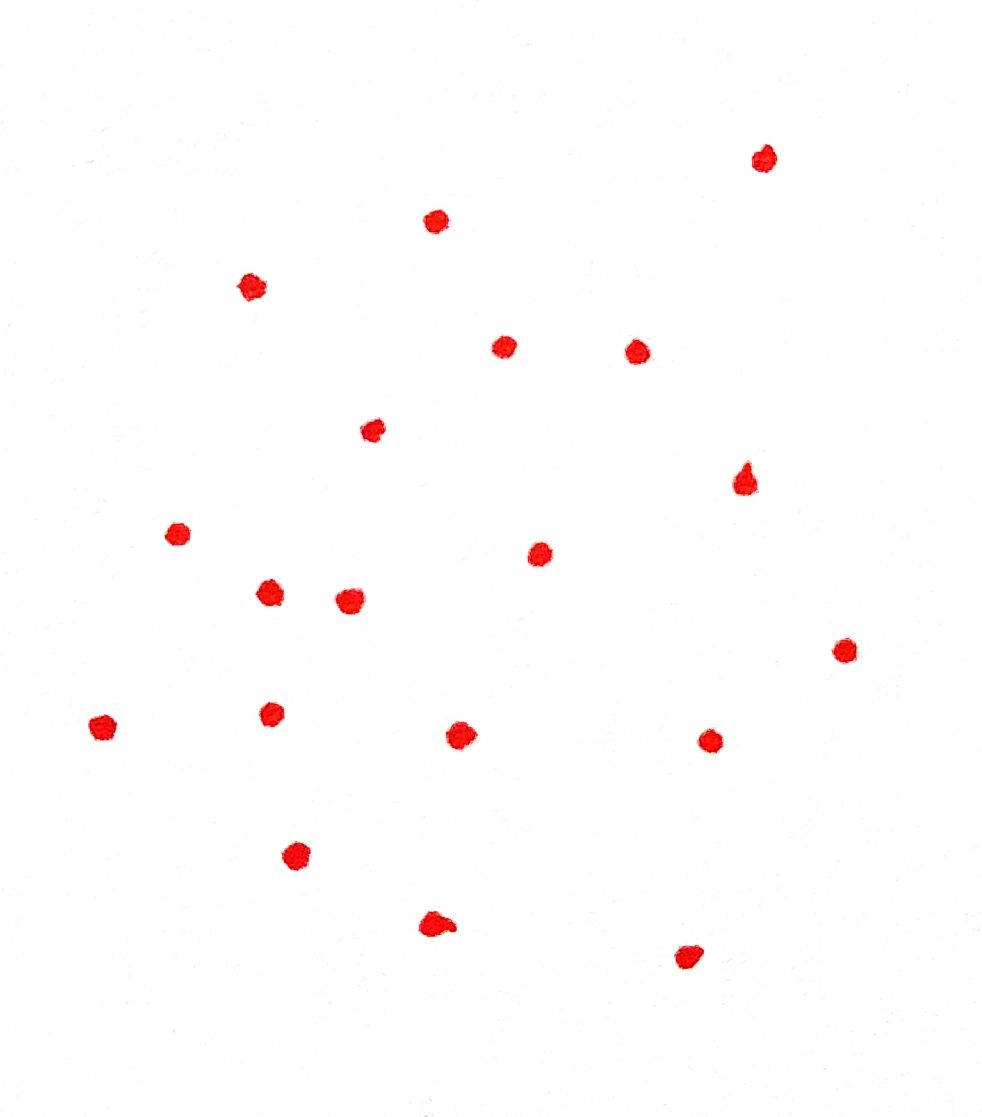
\includegraphics[width=3cm]{convex_hull_input.jpg}
  \end{center}
\end{frame}

\begin{frame} \frametitle{Graham Scan Greedy Heuristic}
\begin{itemize}
  \item $p_1, \ldots, p_m = Q$ sorted into counter-clockwise order, eliminating ties
  \item stack $S$ of points; contains hull of points visited \emph{already}
  \item base case: push first 3 points onto $S$
  \begin{itemize}
    \item for any three points $p, q, r$ forming a non-degenerate triangle,
      $CH(\{p, q, r\}) = \{p, q, r\}$
    \end{itemize}
  \item inductive case:
    \begin{itemize}
      \item examine next input point $p_i$, top of stack $t$, next-lowest stack point $r$
      \item if $\angle r t p_i$ is not a left turn $\implies t$ not on hull
    \end{itemize}
  \item Note: need stack data structure w/ accessor to top \textbf{two} elements
  \end{itemize}
\end{frame}

\begin{frame} \frametitle{Graham Scan Pseudocode}
  {\small
\begin{algorithmic}[1]
  \Function{GRAHAM-SCAN}{$Q$} \Comment{guaranteed $|Q| \geq 3$}
    \State $p_0 = $ lowest point in $Q$ (break ties by choosing leftmost point)
    \State $p_1 \ldots p_m = $ sort $Q-\{p_0\}$ into counter-clockwise order,
      by polar angle with $p_0$; break ties by keeping only the point farthest from $p_0$
    \State $S$ = new stack
    \State $S.PUSH(p0)$
    \State $S.PUSH(p1)$
    \State $S.PUSH(p2)$
    \For { $i$ from $3$ through $m$ }
      \While { $\angle S.BELOWTOP, S.TOP, p_i$ is non-left turn }
        \State $S.POP()$
      \EndWhile
      \State $S.PUSH(p_i)$
    \EndFor
    \State \Return set of point still in $S$
  \EndFunction
\end{algorithmic}
}
\end{frame}

\begin{frame} \frametitle{Graham Scan Analysis}
\begin{itemize}
  \item find $p_0$: $\Theta(n)$
  \item sort: $\Theta(n \log n)$
  \item eliminate tied points: $\Theta(n)$
  \item each stack operation is $\Theta(1)$
  \item \textbf{for} loop repeats $m < n$ times
  \item turn angle test, stack operations are $\Theta(1)$
  \item $\Rightarrow \Theta(n \log n)$ time
  \item dominating term is sort \emph{(reduction to sorting)}
  \item organizing data structure is arrayed stack
  \item $\Rightarrow$ good constant factors
\end{itemize}
\end{frame}

\begin{frame} \frametitle{Jarvis March}
\textbf{Alternative greedy heuristic}: moving around the hull counter-clockwise,
 each step from one vertex to the next is
 \emph{the input point whose angle is shallowest.} \stanza

 $\Rightarrow$ we can start from a $CH$ point, then incrementally find one more $CH$
 point until we're done. \stanza

 Called ``gift wrapping'' b/c this resembles carefully wrapping up an irregular
 object in paper or foil. \stanza 

 (Jarvis march is sometimes called the \emph{gift-wrapping algorithm.})
\end{frame}

\begin{frame} \frametitle{Jarvis March}
  \begin{center}
    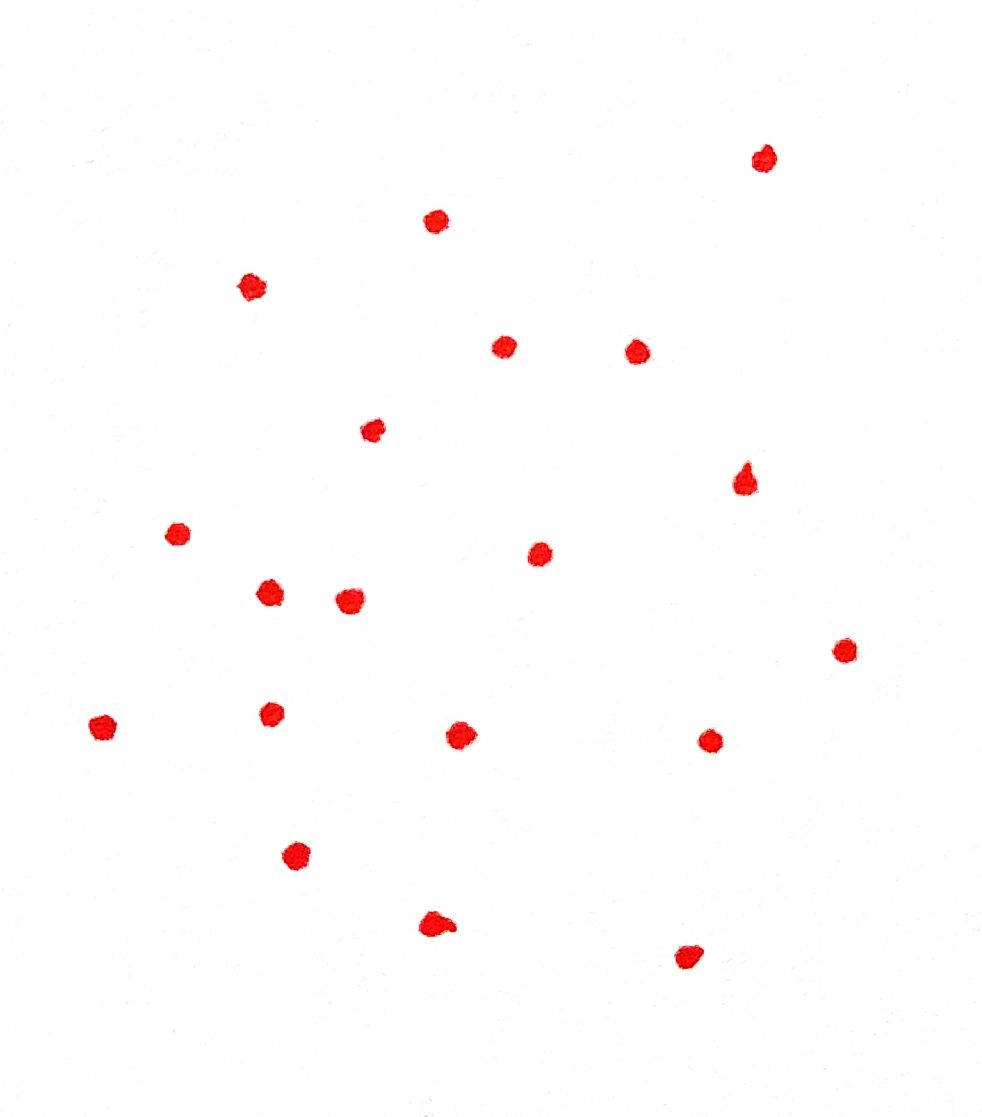
\includegraphics[width=4cm]{convex_hull_input.jpg}
  \end{center}
\end{frame}

\begin{frame} \frametitle{Jarvis March Pseudocode}
Jarvis march $(Q)$
\begin{enumerate}
  \item $H = \emptyset$
  \item Let $\ell = $ lowest point in $Q$ (min. $y$-coord.)
  \item Let $h = $ highest point in $Q$
  \item (right chain) Starting from $\ell$ and until we reach $h$:
    \begin{enumerate}
      \item Linear search $Q$ for the next point $p_i$, minimizing the angle
        between $p_i$ and the previous point
      \item Include $p_i$ in $H$ and continue the loop at $p_i$.
    \end{enumerate}
  \item (left chain) Repeat the previous process but starting from $h$ and ending at $\ell$.
  \item Return $H$
\end{enumerate}
\end{frame}

\begin{frame} \frametitle{Jarvis March Analysis}
  Preprocessing to find $h, \ell: \Theta(n)$ \stanza

  Each iteration of the left/right-chain loops identifies one hull point \\
  $\implies$ in total they iterate $h$ times,
  where $h \equiv $ number of points on the hull. \stanza

  linear search inside the loops takes $\Theta(n)$ time. \stanza

  $\therefore$ $\Theta(nh)$ total time. \stanza
\end{frame}


\begin{frame} \frametitle{Comparison of Convex Hull Algorithms}
\begin{center}
  \begin{tabular}{|l|l|l|}
    \hline
    \textbf{Algorithm} & \textbf{Time} & \textbf{Main Idea} \\ \hline
    Graham Scan & $\Theta(n \log n)$ & sort, skip right turns \\
    Jarvis March & $\Theta(nh)$ & gift-wrapping \\
    \hline
  \end{tabular}
\end{center}
\vspace{.5cm}
What is the relationship between $n$ and $h$?
\end{frame}

\begin{frame} \frametitle{$n$ vs $h$}
  Recall
  \begin{itemize}
    \item $n \equiv $ \# input points $= |Q|$
    \item $h \equiv $ \# output points $=$ \# vertices of convex hull $= |CH(Q)|$
    \stanza
  \end{itemize}

  For fixed $n,$
  \begin{itemize}
    \item minimum $h = 3$ when all input points are enclosed in a triangle
    \item maximum $h = n$ when all input points happen to be convex hull vertices
    \item $ 3 \leq h \leq n $
  \end{itemize}

  \begin{center}
    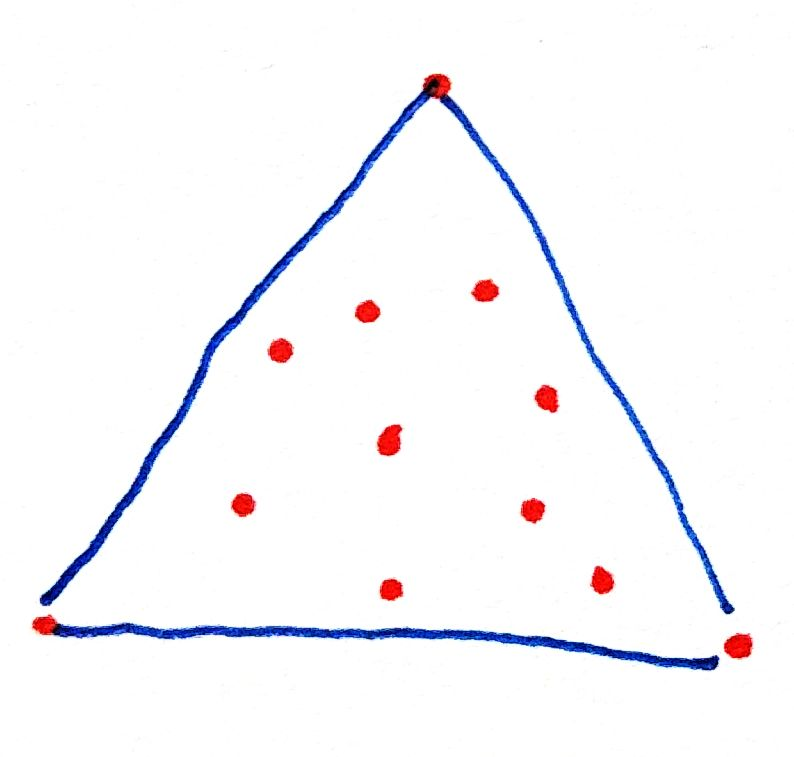
\includegraphics[width=2cm]{convex_hull_smallest_output.jpg}
    \hspace{.5cm}
    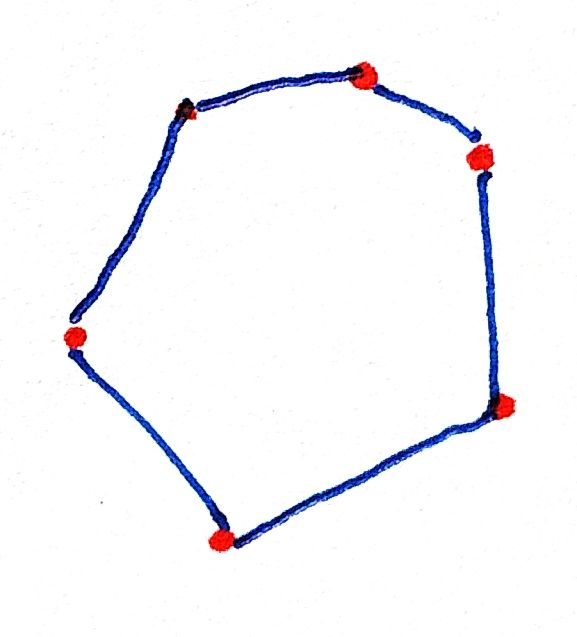
\includegraphics[width=2cm]{convex_hull_largest_output.jpg}
  \end{center}

\end{frame}

\begin{frame} \frametitle{Summary of Convex Hull Algorithms}
  FYI
  \begin{itemize}
    \item \textbf{Chan's algorithm} is an optimal output-sensitive algorithm
    \item (not covered in book or class)
    \item combines both algorithms, divides input points using Graham's heuristic,
      merges hulls using Jarvis' heuristic
    \item $\Theta(n \log h)$ time \stanza
  \end{itemize}

\begin{center}
  \begin{tabular}{|l|l|l|l|}
    \hline
    \textbf{Algorithm} & \textbf{Time} & $h \in O(1)$ & $h \in \Theta(n)$ \\ \hline
    Graham Scan & $\Theta(n \log n)$ & $\Theta(n \log n)$ & $\Theta(n \log n)$ \\
    Jarvis March & $\Theta(nh)$ & $\Theta(n)$ & $\Theta(n^2)$ \\
    Chan's algorithm & $\Theta(n \log h)$ & $\Theta(n)$ & $\Theta(n \log n)$ \\
    \hline
  \end{tabular}
\end{center}

\end{frame}

\end{document}
